%%%%%%%%%%%%%%%%%%%%%%%%%%%%%%%%%%%%%%%%%
% University/School Laboratory Report
% LaTeX Template
% Version 3.0 (4/2/13)
%
% This template has been downloaded from:
% http://www.LaTeXTemplates.com
%
% Original author:
% Linux and Unix Users Group at Virginia Tech Wiki 
% (https://vtluug.org/wiki/Example_LaTeX_chem_lab_report)
%
% License:
% CC BY-NC-SA 3.0 (http://creativecommons.org/licenses/by-nc-sa/3.0/)
%
%%%%%%%%%%%%%%%%%%%%%%%%%%%%%%%%%%%%%%%%%

%----------------------------------------------------------------------------------------
%	PACKAGES AND DOCUMENT CONFIGURATIONS
%----------------------------------------------------------------------------------------

\documentclass{article}

\usepackage[version=3]{mhchem} % Package for chemical equation typesetting
\usepackage{siunitx} % Provides the \SI{}{} command for typesetting SI units

\usepackage{graphicx} % Required for the inclusion of images
\usepackage{caption}
\usepackage{subcaption}
\usepackage{cancel}

\usepackage{float}

\usepackage[T1]{fontenc} % allow small bold caps

\usepackage{titlesec}

\usepackage{enumitem}

\setcounter{secnumdepth}{4}

\titleformat{\paragraph}
{\normalfont\normalsize\bfseries}{\theparagraph}{1em}{}
\titlespacing*{\paragraph}
{0pt}{3.25ex plus 1ex minus .2ex}{1.5ex plus .2ex}

\setlength\parindent{0pt} % Removes all indentation from paragraphs

\renewcommand{\labelenumi}{\alph{enumi}.} % Make numbering in the enumerate environment by letter rather than number (e.g. section 6)

%\usepackage{times} % Uncomment to use the Times New Roman font

%----------------------------------------------------------------------------------------
%	DOCUMENT INFORMATION
%----------------------------------------------------------------------------------------

\title{Machine Learning and Pattern Analysis for Identification of Lung Sounds\\ UAP Report} % Title

\author{Ryan Lacey}

\date{}

\begin{document}

\maketitle % Insert the title, author and date

\begin{center}
\begin{tabular}{l r}
Advisor: & Dr. Rich Fletcher \\
\end{tabular}
\end{center}

\section{Background and Motivation}

Pulmonary diseases (asthma, pneumonia, lung cancer, tuberculosis, etc.) are an increasing concern in the realm of global health challenges. Chronic obstructive pulmonary disease (COPD) alone is currently the third leading cause of death in the world and second leading cause of death in India. Pneumonia, which also affects the lungs, remains the leading cause of death in Indian children under the age of five. Especially at risk are low income populations due to consequences of living environment, lack of access to health care, and the high cost of screening tools for detection of these diseases.\\

There is a great need to provide health workers in India a simple tool that can be used to screen for respiratory disease in the primary care setting and identify individuals that require clinical examination and intervention. Since a majority of the clinicians practice Ayuverdic medicine they have little training for diagnosing respiratory problems. As a result many patients go undiagnosed or are misdiagnosed with having a cardiac disease. The disease burden can be significantly reduced if there were better tools that could perform early detection of respiratory disease and enable clinical intervention before the disease became more critical or developed further into chronic disease. \cite{Fletcher}\\

\section{Scope of the Project}

The overall goal of project is to develop a mobile application for use in clinics with limited resources in developing regions of India. The application shall serve as a diagnostic tool for clinicians trained in Ayuverdic medicine to diagnose patients suffering from a pulmonary disease. With an Android mobile device and a low cost digital stethoscope these clinicians will be able to collect patient lung sounds, run diagnostic machine learning algorithms on the lung sound data, and receive classification feedback with the objective of early detection of the onset of pulmonary disease. \\

 Based on feedback from our clinical partners, and in order to maintain better confidence in the algorithm, we shall employ sound features that are also used in standard clinical pulmonary diagnostic procedure. These basic lung sounds include: crackle, wheeze, and plural rub. Using recorded acoustic samples, we shall apply a pattern recognition algorithm to optimize the detection of these specific features at the different locations on the body. Therefore, rather than performing disease classification directly from the raw sound files, we have decided to separate the software into two parts, as shown below: \\
 
 \begin{figure}[H]
 \minipage{\textwidth}
 	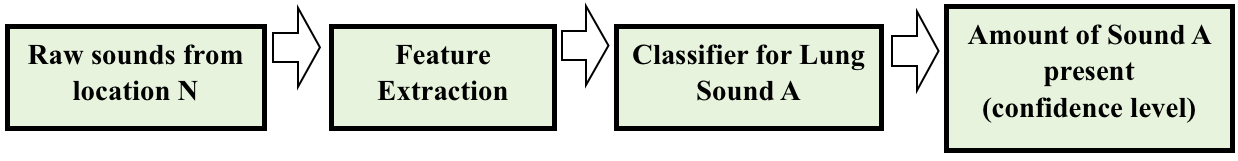
\includegraphics[width=\linewidth]{images/SoftwareGoal1.png}
 	\caption{Software goal 1 -- sound identification}
 \endminipage\hfill
 \end{figure}
 
 This section of software applied pattern recognition algorithms and machine learning to estimate how much of each type of lung sound is present in the sample sound file.  Since the amount of lung sound present is generally a subjective assessment performed by a human doctor, this portion of software involves its own machine learning algorithm to produce outputs in the form of estimates (confidence levels).  This software can be tested and validated separately against the results from a trained pulmonologist.\\
 
 Once we have calculated the amount of specific lung sounds present in each sample, from each location on the body, a second machine learning algorithm can be applied to perform the actual diagnosis.\\
 
  \begin{figure}[H]
  \minipage{\textwidth}
  	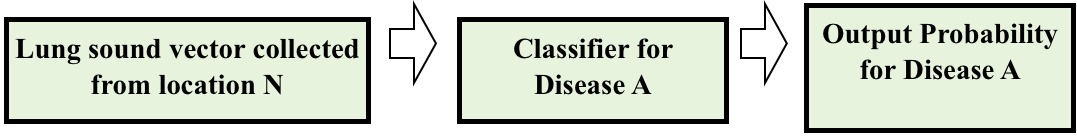
\includegraphics[width=\linewidth]{images/SoftwareGoal2.png}
  	\caption{Software goal 2 -- sound diagnosis}
  \endminipage\hfill
  \end{figure}

  For this project, I am focusing on part one of the software, with the goal of identifying the amount of each lung sound present in the sound files.\\
  
\section{Lung Sounds}

Three types of lung sounds are used in the diagnosis of pulmonary disease: wheeze, crackle, and pleural rub. 

\subsection{Wheeze}

Wheeze is characterized by a set of sustained musical sounds caused by restricted airflow from a narrow or blocked passage. More blocked passages tends to correlate with an increase in wheezes, but extreme blockage can restrict airflow to the point that no wheeze may be heard. Wheezes can be heard in either inhalation or exhalation. Multiple frequencies can be heard in these sounds.  Several clinical organizations have divided sounds into  two categories: high frequency wheeze and low frequency wheeze. High frequency wheezes are produced by the upper parts of the respiratory system, while low frequency wheezes are produced by the lower parts. 

\subsection{Crackle}

Crackle is characterized by short, non-musical, explosive sounds from the either the mouth or chest. A typical crackle lasts approximately 20 ms. There are two main sub-classifications of crackle: coarse and fine. Coarse crackles are heard earlier in inspiration and throughout expiration. They indicate that the airway is only open intermittently and may be related to secretions. Fine crackles are heard later in the inspiration cycle and occasionally through expiration. They are unrelated to secretions and are often one of the earliest signs of disease. Only coarse crackles may be transmitted to the mouth. \cite{Yi MEng, NEJoM}.

\subsection{Pleural Rub}

Pleural rub is characterized by low-pitched, grating, or creaking sounds. The sounds are caused by pleural surfaces rubbing together during the respiratory cycle. The rubbing indicates the presence of pleural inflammation or tumors. Pleural rub can be heard during inhalation or exhalation, but is more common in the former. \cite{rnceus}

\newpage

\section{Software Implementation}

\subsection{Software Tools}

 With the goal of machine learning classification in mind, the first task was to determine what tools were to be used on the lung data. \\
 
 The most fundamental function of the application is for machine learning algorithms to give a binary classification of the data, ie. either the patient has the disease or the patient does not suffer from the disease. Since these classifiers only state "yes or no" instead of "which", each disease will require its own classifier. The most common technique for this type of classification is a linear classifier called a support vector machine (SVM). The SVM will train on pre-classified data of Indian patients with the target diseases and aims to minimize potential misclassification of future patients based off of the sample data. Since there are no known machine learning libraries for Android devices, a large portion of the work for this project will be in the implementation, training, and testing of these algorithms.\\
 
 I investigated several machine learning libraries available in Java including: Weka, Mallet, and LibSVM. Each of the options, however, had drawbacks that were cause for hesitation. Weka is a comprehensive suite of machine learning algorithms and data mining tools. The software is one of the most popular machine learning packages available and is available into both an executable form to run on pre-formatted data as well as a developers version that can be modified for specific needs. Unfortunately the documentation for the software was rather difficult to traverse and contained a large host of functionalities that both were outside of the scope of the needs of classification and outside of my knowledge in machine learning. Since the timescale for this project was so limited, I wanted to minimize the ramp up time of learning and integrating a complex library, which made this option unattractive. Additionally investigation revealed that potential issues would arise in porting the Weka code to Android, so the long-term use of the software was in question. Mallet was attractive initially because its documentation was more comprehensible and easier to navigate than that Weka provided. However it advertises itself as a package for natural language processing and document classification, which is a large field utilizing techniques not necessarily applicable to the lung sound data. The final consideration, LibSVM, is Java software ported from a popular C package of the same name. Therefore the limited supporting documentation was written in C, which I have no experience with, and had difficulty parsing. \cite{Weka, Mallet} \\
 \\
 
 The lack of clear documentation, potential trouble in porting from Java to Android, and concerns over underutilization of software features at a great cost to system resources called into question the benefit of using a machine learning library. I had previously implemented classification algorithms in a machine learning course that I was concurrently enrolled in and pushed forward the idea of doing the algorithms myself for this project. This involved three steps: creating a working classifier, implementing the SVM algorithm, and running classifications on lung data.\\
 
 My first task was to implement the perceptron algorithm -- a simple, but widely used classifier. I had written this before in Python for use in classification of data from Twitter, so conversion to Java was relatively straightforward. The Java implementation was ran on the same Twitter data as a check for correctness, since the performance should have been comparable to the Python code. In regards to the classifier itself the only challenge was performance. The mathematics behind the algorithm is heavily dependent upon multidimensional matrix manipulations. Traditional looping constructs, although viable for correctness, would have yielded a product virtually unusable due to computation time. The Python code addressed this by using the Numpy library. I researched for a comparable linear algebra toolkit in Java and settled on the Apache Commons Mathematics Library. With efficient matricies at hand, I wrote several parsers for formatting the Twitter data and extracting features to classify on. The classifier was tested on a pre-labeled set of test tweets and correctly labeled over 85\% of the points. Thus a basic classifier was available for any data set.\\
 
 The code was structured so that pieces may be swapped out easily. The three main components were the parsers to read in data, algorithms to construct a feature matrix from the data, and the machine learning algorithm to classify the data. The second task was to implement the more powerful SVM classifier. The SVM algorithm is similar to perceptron in that they are both linear classifiers. The advantage of the SVM, however, is that it is a maximum margin separator. This means that the classification line will pass through the point that maximizes the distance between the nearest oppositely labeled training data points. If the line passed closer to one of the data points, then the likelihood that the classifier overfits the data increases. Overfitting gives good results on testing data but has the tendency to generalize poorly to test data in the general population.\\
 
 At this stage SVMs had just been covered in the machine learning course. The techiques for implementing a SVM were very different from the perceptron algorithm and required linear solvers. It became apparent that implementing this myself was not optimal because it would have required yet another library to be brought in to the project and forseeably a great undertaking in working out all of the details of the algorithm. Thus I decided to return to incorporating a machine learning library, specifically LibSVM. The modular structure of the existing code made integration of the library's SVM a smooth process with minimal changes. Use of the library also awarded additional functionality, including confidence intervals for the SVM. These are values in the range [0,1] attributing how much the classifier associates test data with each label. With a SVM in hand the focus of the project switched to classification on the lung data. \cite{SVM}\\

\subsection{Feature Extraction}

Feature extraction was the most open ended and challenging  component of the project. Since Android devices have limited processing power due to their mobile processing cores a balance was struck between having enough features to be able to separate lung conditions while keeping computational demand at a minimum. The features should not only correctly classify lung sounds, but also do so with a high degree of confidence. \\

\begin{figure}[h!]
	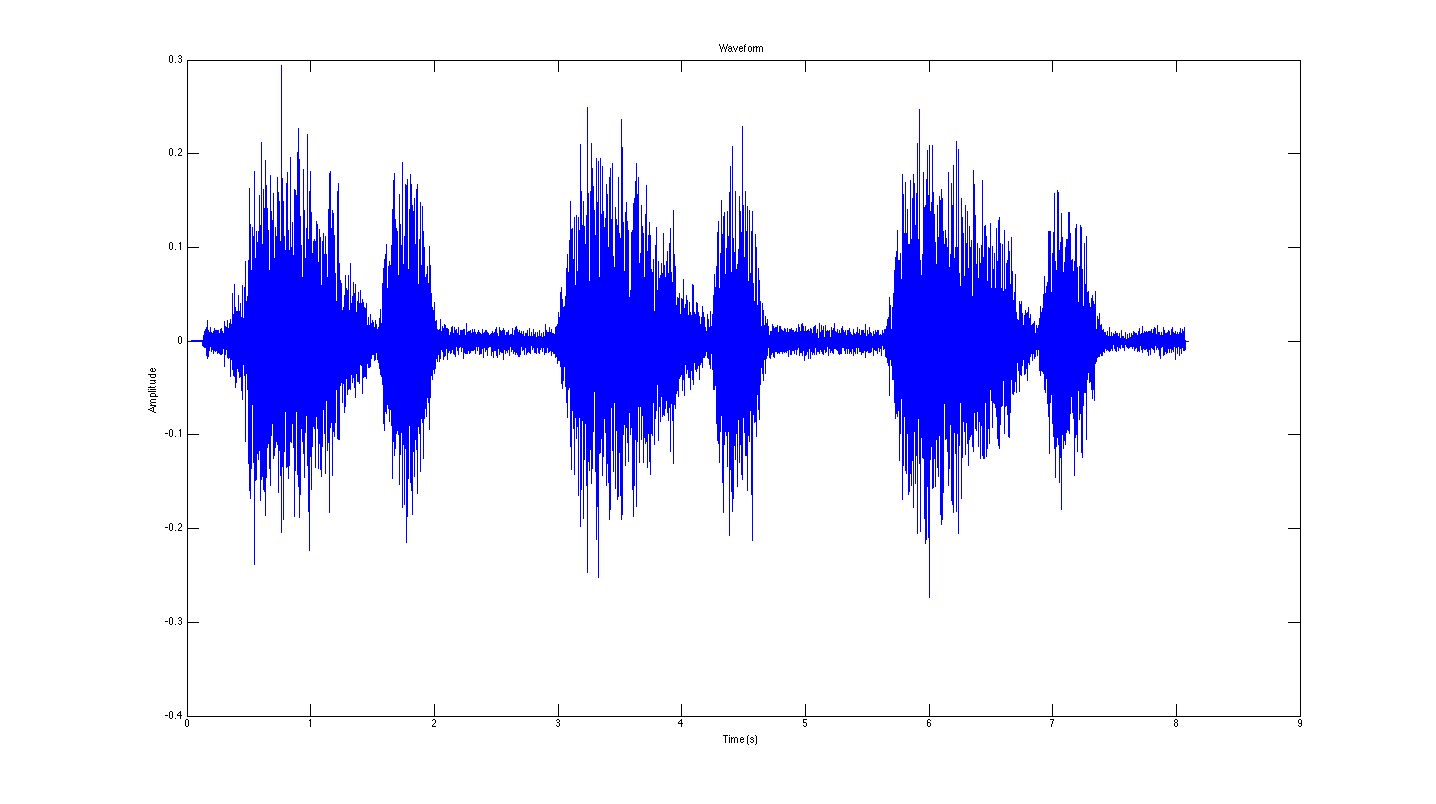
\includegraphics[width=\linewidth]{images/VesicularWaveform.png}
	\caption{Waveform of vesicular lung sound}
 	\label{fig:VesicularWaveform}
\end{figure}

Lung data comes in the form of an audio file represented by signal amplitude taken at regular intervals determined by the sampling frequency. A graph of amplitude over time represents the waveform of the lung sound, as seen in Figure \ref{fig:VesicularWaveform}. From the waveform one can see the cycles of inhalation and exhalation, which are the pairs of high amplitude signals separated by low amplitude lulls between breaths. \\
\newpage
\subsubsection{Wheeze}

\paragraph{Characteristics}

Lung wheeze is characterized by well-defined pitches over sustained durations. To observe the pitch characteristics the signal is tranformed from the time domain to the frequency domain through a Fast Fourier Transform. Clinicians categorize wheeze into two types: low wheeze and high wheeze. These wheezes, respectively, have large magnitude peaks in low frequency (<200 Hz) and higher frequency (>400 Hz) regions. Figure \ref{fig:FFTVesicularWheeze} overlays a vesicular and high pitch wheeze in the frequency domain. The low frequency portions of the signals do not show an appreciable difference in magnitude. The high frequency signal magnitudes, on the other hand, differ greatly. The vesicular signal has a gradual and relatively constant decrease in magnitude moving into the higher frequencies. In contrast the wheeze signal has a very large magnitude peak that is approximately four times greater than strongest frequency signal of the vesicular data. \\

\begin{figure}[H]
	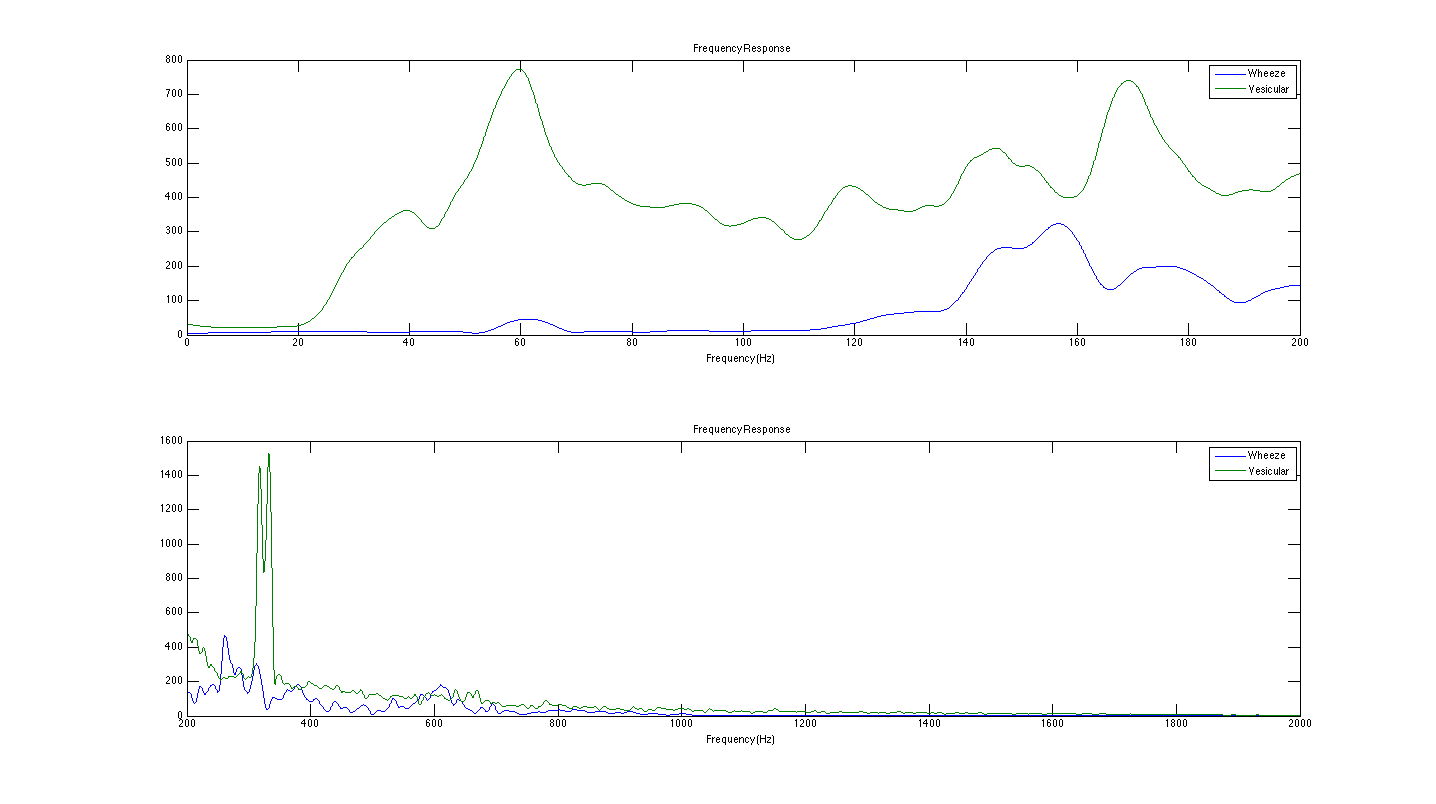
\includegraphics[width=\linewidth]{images/FFTVesicularWheeze.png}
	\caption{Comparison of vesicular and high pitched wheeze in frequency domain}
 	\label{fig:FFTVesicularWheeze}
\end{figure}

\paragraph{Features}

\begin{itemize}[noitemsep,nolistsep]
\item
	Peak frequency in midrange frequency region (250-800 Hz)\\
\item
	Ratio of max signal amplitude in midrange frequency region to average signal amplitude in midrange frequency region\\
\item
	Ratio of signal amplitudes across low frequency region to middle frequency region\\
\item
	Ratio of signal amplitudes across high frequency region to middle frequency region\\
\item
	Area under the curve of low frequency region normalized to maximum frequency in low region\\
\item
	Area under the curve of midrange frequency region normalized to maximum frequency in midrange region\\
\item
	Area under the curve of high frequency region normalized to maximum frequency in high region\\
\item
	Sliding window wheeze count (see \ref{Wheeze Sliding Window})\\
\end{itemize}

\paragraph{Sliding Window Count}\label{Wheeze Sliding Window}

The identifying traits of wheeze sounds are not persistent, so the time domain signal is discretized into 300 ms blocks for detection of these characteristics. The technique for identifying wheeze components in a lung sound was drawn from the wheeze detector algorithm of \cite{Yi MEng}. A 300 ms window was chosen because The American Thoracic Society defines the minimum duration of a wheeze to be 250 ms. Therefore this encapsulates the entire waveform with tolerance for deviation from the average.\\

One can visually identify wheeze by the regular periodic nature of the signal in the time domain. The frequency of the signal over these spans is the fundamental frequency. An example of the regular nature of a wheeze signal component is shown in Figure \ref{fig:WheezePeriodicity}. This contrasts sharply with the random and irregular progression of the time domain signal for non-wheeze components of a wheeze signal and entire signal spans for other lung sounds, as seen in Figure \ref{fig:WheezeRandomness}. Note that these components come from the same signal and are only separated by approximately 500 ms. \\

\begin{figure}[H]
	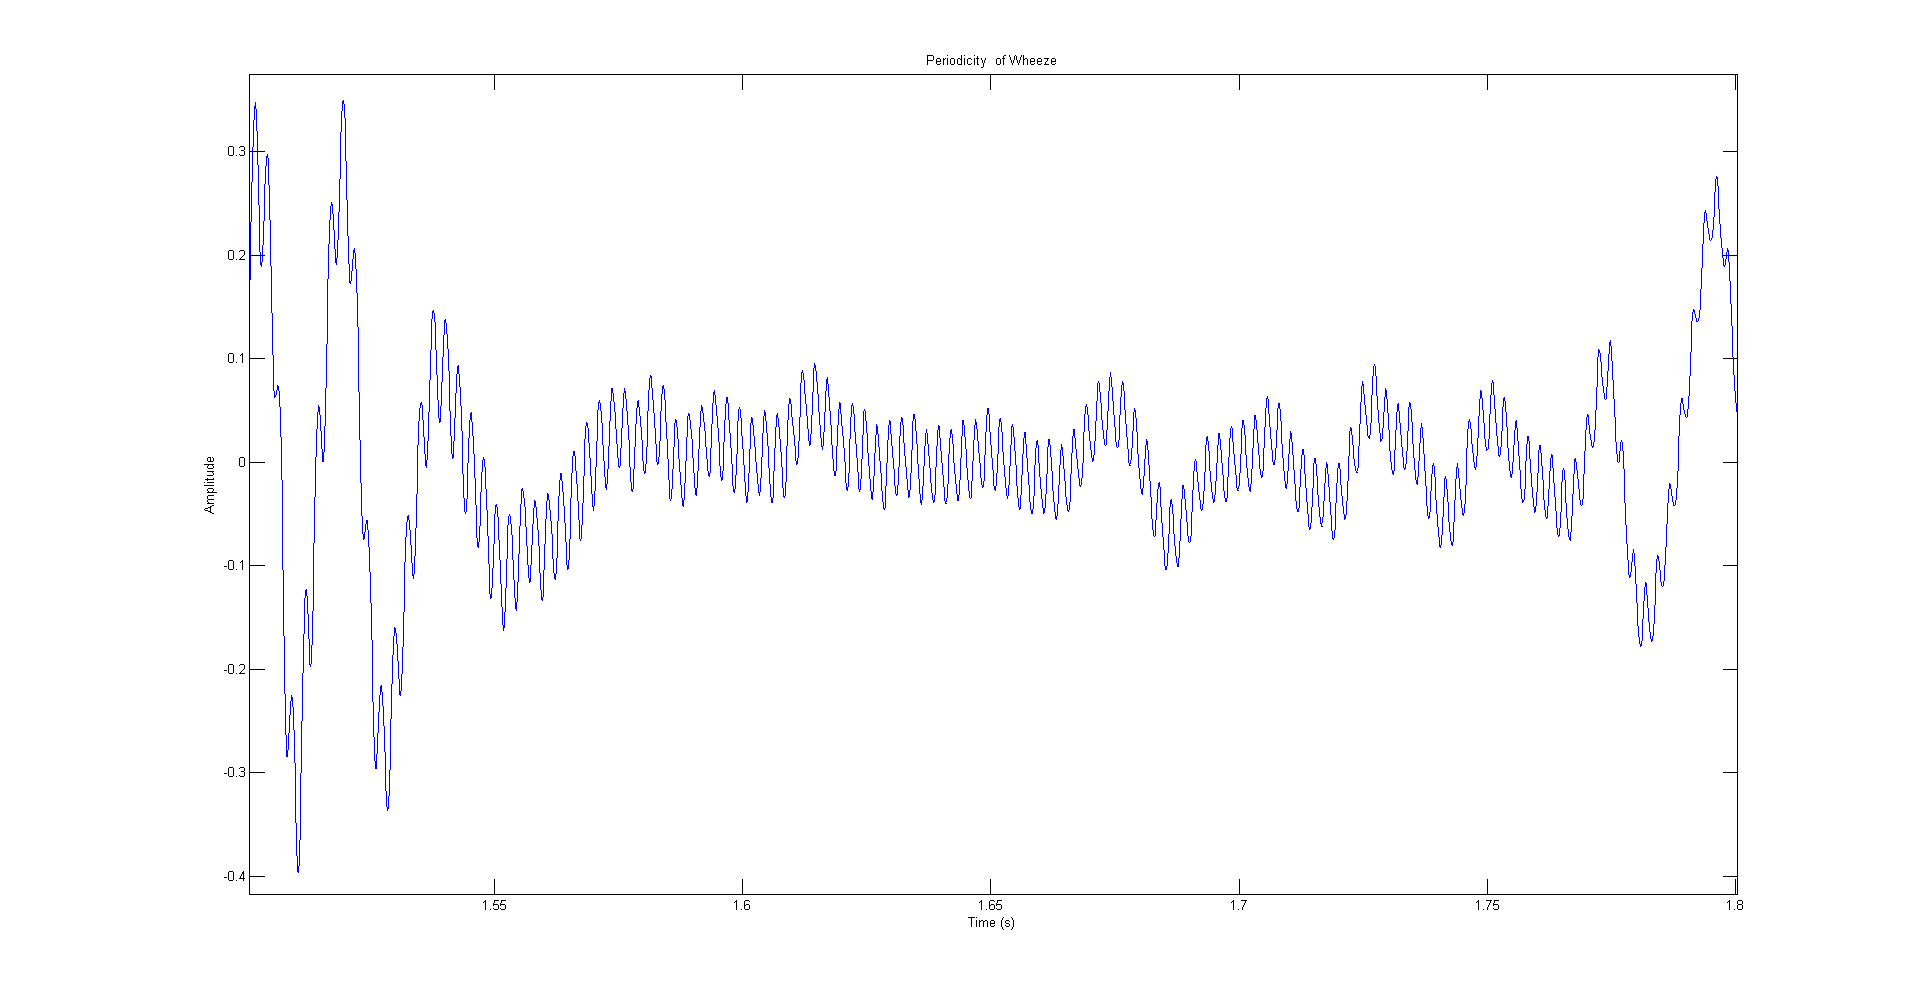
\includegraphics[width=\linewidth]{images/WheezePeriodicity.png}
	\caption{Wheeze component of time domain signal}
 	\label{fig:WheezePeriodicity}
\end{figure}
\begin{figure}[H]
	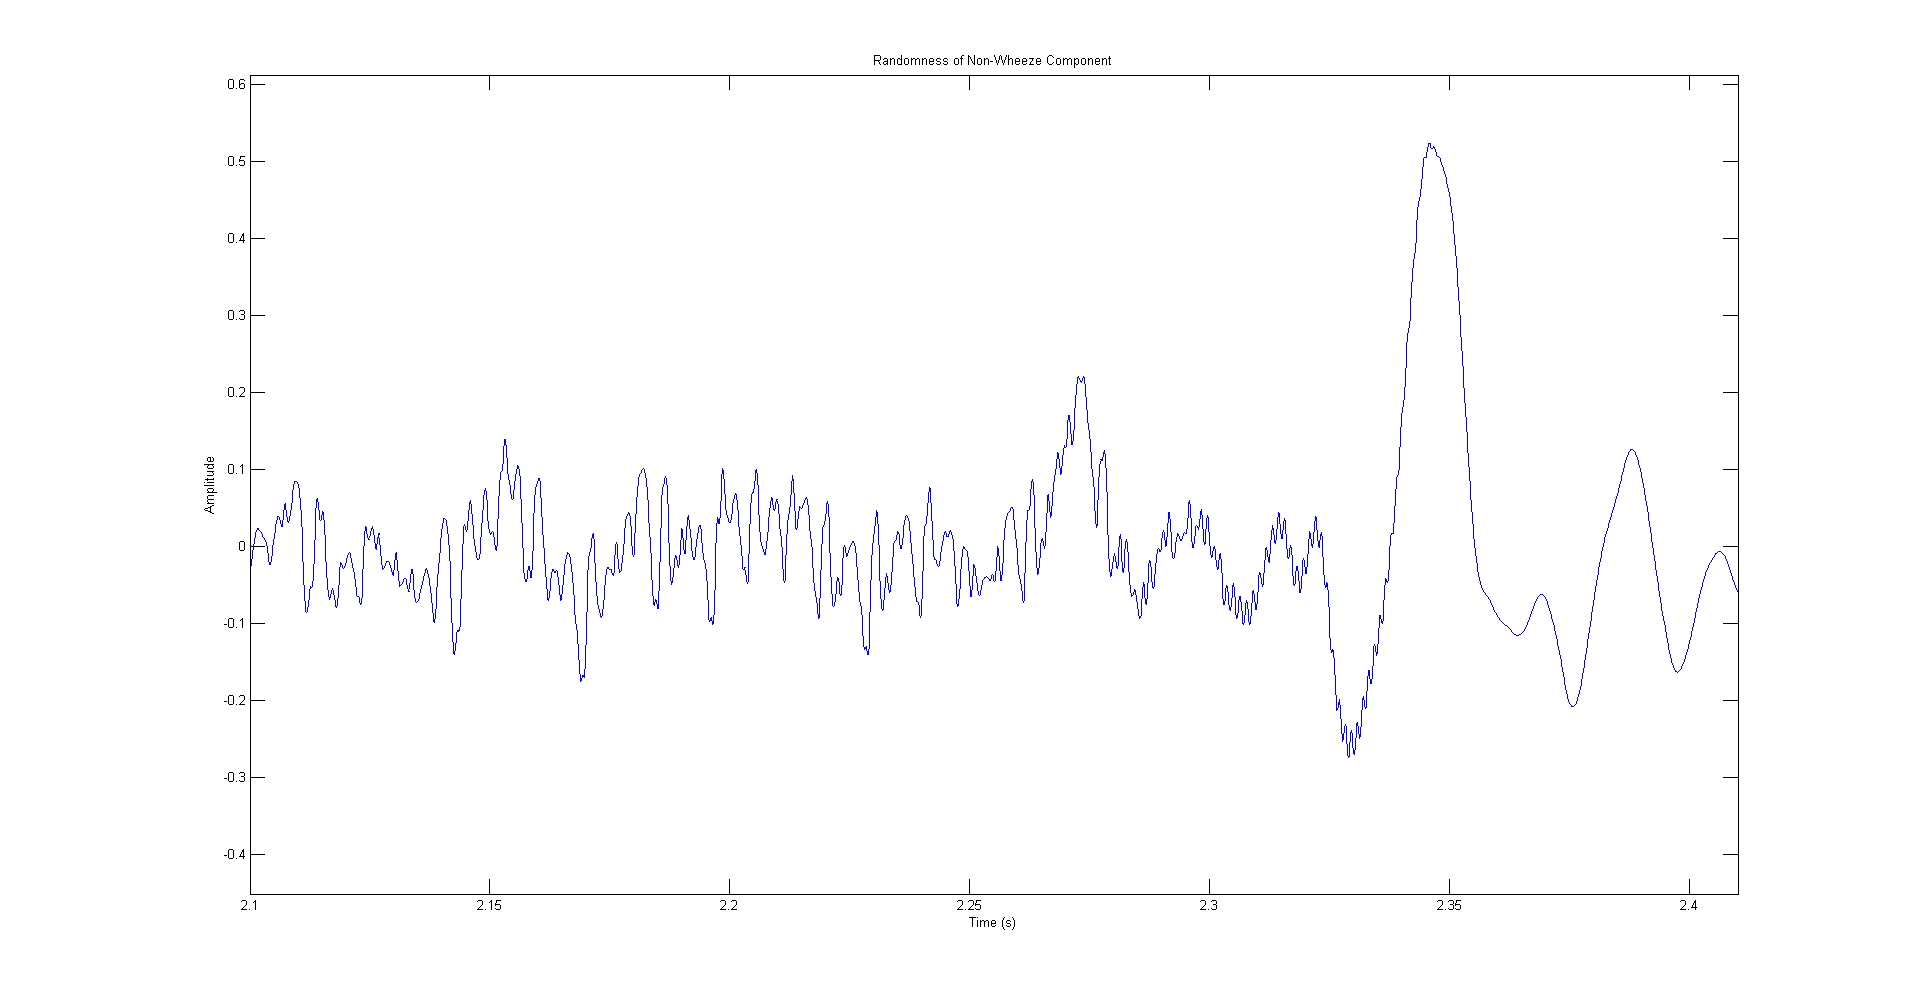
\includegraphics[width=\linewidth]{images/WheezeRandomness.png}
	\caption{Non-wheeze component of time domain signal}
 	\label{fig:WheezeRandomness}
\end{figure}

In each window the time domain signal is transformed into the frequency domain and smoothed to reduce noise. The algorithm is calibrated for high-pitch wheeze detection, so it will look for strong peaks within the 250-600 Hz range. A peak is considered strong if its width spans less than a 160 Hz range and if the base amplitude of the signal is at most 15\% of the maximum amplitude. A count of strong peaks is output after iterating over the entire audio file in increments of 150 ms. The incremental step size is half of the window size so that any peak partially captured by one window is fully realized in the next.\\

\subsubsection{Crackle}

\paragraph{Characteristics}

Crackle is characterized by spikes in signal amplitude in the time domain. The magnitude of the spikes tends to be much greater than the maximums normally observed in inspiration and expiration. Observe the crackle waveform of Figure \ref{fig:CrackleWaveform} and compare it to the vesicular waveform of Figure \ref{fig:VesicularWaveform}. Note that the crackle induced spikes in signal amplitude are approximately four times as strong as the peaks across the normal components of the lung sound.\\

\begin{figure}[H]
	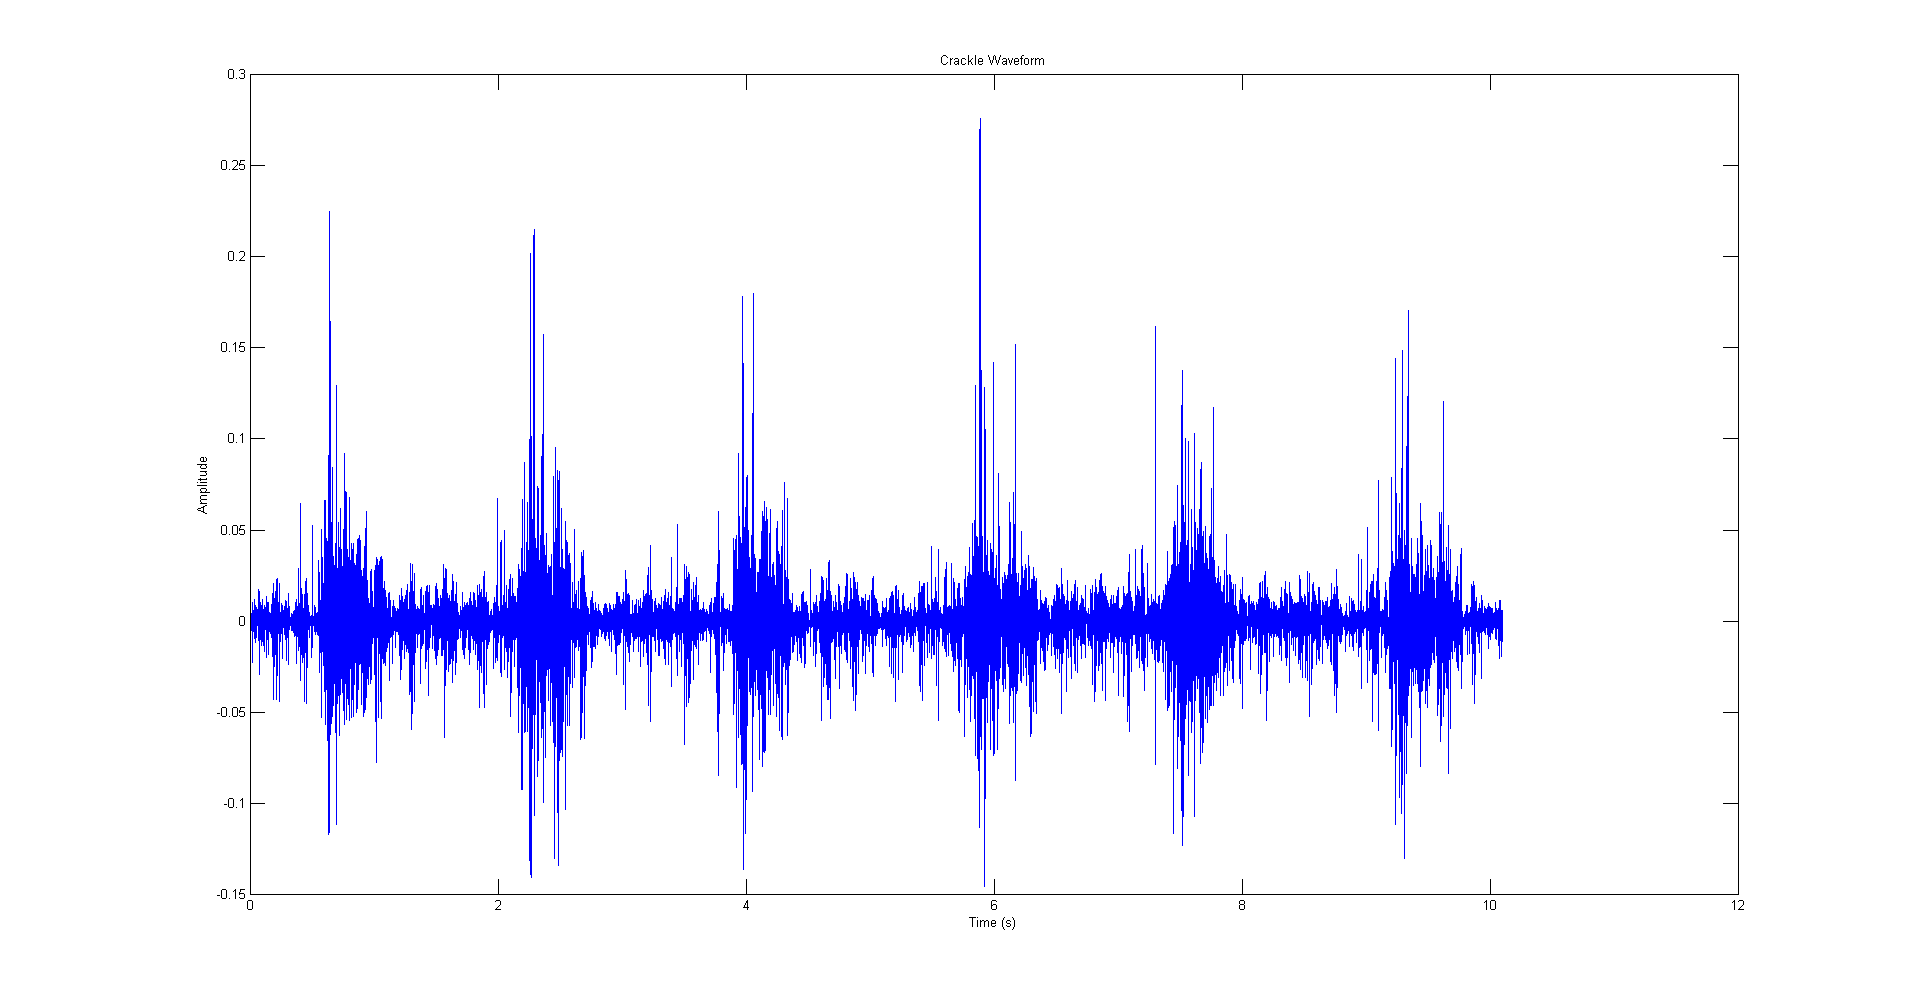
\includegraphics[width=\linewidth]{images/CrackleWaveform.png}
	\caption{Waveform of crackle lung sound}
 	\label{fig:CrackleWaveform}
\end{figure}

\paragraph{Features}

\begin{itemize}[noitemsep,nolistsep]
\item
	Peak frequency in midrange frequency region (250-800 Hz)\\
\item
	Ratio of max signal amplitude in low frequency region to average signal amplitude in low frequency region\\
\item
	Ratio of max signal amplitude in midrange frequency region to average signal amplitude in midrange frequency region\\
\item
	Ratio of max signal amplitude in high frequency region to average signal amplitude in high frequency region\\
\item
	Ratio of signal amplitudes across low frequency region to middle frequency region\\
\item
	Ratio of signal amplitudes across high frequency region to middle frequency region\\
\item
	Area under the curve of low frequency region normalized to maximum frequency in low region\\
\item
	Area under the curve of midrange frequency region normalized to maximum frequency in midrange region\\
\item
	Area under the curve of high frequency region normalized to maximum frequency in high region\\
\item
	Sliding window crackle count (see \ref{Crackle Sliding Window})\\
\end{itemize}

\paragraph{Sliding Window Count}\label{Crackle Sliding Window}

The sliding window technique for crackle is analogous to that used in wheeze detection. The differentiating factor is that crackle peaks are found in the time domain instead of the frequency domain. The burst nature of crackle requires a small window, on the order of 40 ms, in order to capture at most only one peak at a time. A strong peak is defined as having a signal amplitude within 25\% of the maximum amplitude across the entire audio file and a value at least 3.6$\times$ stronger than the average signal in its respective window. As was the case with the wheeze windows, the crackle windows overlap at intervals half of the window width in order to fully capture all peaks in the signal.
\newpage
\section{Results}

The audio files used for training and testing the classifiers consisted of: eight vesicular, eight high-pitched wheeze, and eleven crackle lung sounds. Since the available data was limited, a leave-one-out technique was employed for analyzing the classifiers. Twenty-six of the twenty-seven audio files were used as the training data set, while the remaining file was used as the test data. Each audio file was left out once per classifier, totaling fifty-four trials across the twenty-seven files for the two classifiers. Note that once the classifiers are trained the size of the testing set is irrelevant, so it was optimal to only use one file for testing at a time.\\

Since the true label of each audio file was known, each was ran through both classifiers to determine if the classifier correctly attributed the respective lung condition to the sound. The results were as follows:\\


\begin{align*}
\begin{tabular}{ r|c|c| }
\multicolumn{1}{r}{}
 \emph{Wheeze} & \multicolumn{1}{c}{Positive}
 & \multicolumn{1}{c}{Negative} \\
\cline{2-3}
True & 6 & 0 \\
\cline{2-3}
False & 19 & 2 \\
\cline{2-3}
\end{tabular}
\end{align*}

\begin{align*}
\begin{tabular}{ r|c|c| }
\multicolumn{1}{r}{}
 \emph{Crackle} & \multicolumn{1}{c}{Positive}
 & \multicolumn{1}{c}{Negative} \\
\cline{2-3}
True & 9 & 1 \\
\cline{2-3}
False & 15 & 2 \\
\cline{2-3}
\end{tabular}
\end{align*}

In summary:
\begin{itemize}
\item
	$\dfrac{49}{54}\approx 91\%$ of all classifications were correct
\item
	$100\%$ of wheeze and $90\%$ of crackle classifications were for sounds that actually had those symptoms
\item
	$75\%$ of wheeze sounds and $82\%$ of crackle sounds were found by their respective classifiers
\end{itemize}

Not shown in the graphs:
\begin{itemize}
\item
	Average confidence in prediction of found wheezes was $92\%$\\
	Average confidence including misclassified wheezes was $79\%$
\item
	Average confidence in prediction of found crackles was $76\%$\\
	Average confidence including misclassified crackles was $64\%$
\end{itemize}

\newpage

\section{Conclusion and Future Work}

Two objectives defined this project: to correctly classify lung sounds and to do so with great confidence. The results demonstrate that both of these goals were met. The classifiers were very accurate when claiming that a sound had pulmonary ailments. While the confidence of $76\%$ for crackle potentially leaves room for doubt in the classification, the $92\%$ average confidence of the wheeze classifier is rather phenomenal. Thus if the wheeze classifiers output positive for a patient, clinicians should have a strong inclination to believe that the patient truly has that condition.\\

Although the high accuracy and confidence in true positives gives promise for field application, the false negatives leave room for future improvements. For this project, with such a limited dataset, a balance had to be struck between capturing a condition with its respective qualifier without also incorrectly attributing the condition to lung sounds that were not actually affected. Naturally a larger training set should improve the classifiers as they will have a better sense of the population. This should improve their ability in general applications and on data that is not as well structured as the files used for this project, which were strong examples of their respective lung sound conditions.\\

The most open ended question for future work remains which features should be included to represent each lung sound. Too many features increases strain on the mobile processor and has a tendency towards overfitting. Too few features may lead to poor differentiation between different lung sounds and thus poor generalization to the population. While unquestionably there are certain features that should be targeted when classifying specific sounds (eg. frequency domain for wheeze), to some degree the process is guided by trial and error. Even with the small set of features chosen for this project there is a large degree of freedom in choosing various thresholds. For instance a change of 5\% in the threshold value for frequency peaks in the wheeze sliding window resulted in nearly a 10\% average gain in confidence for classifications. It is difficult to say how much more the parameters chosen can be similarly optimized and how much there is to gain from additional features being added to the classifiers.\\

\newpage

\begin{thebibliography}{9}
\bibitem{Fletcher}
	Fletcher, Richard, PhD. Low-Cost Mobile Diagnostic Tools for Pulmonary Disease. Tech. Cambridge: MIT D-Lab and Media Lab, 2013. Print.
\bibitem{Yi MEng}
	Yi, Gina A., and John V. Guttag. A Software Toolkit for Acoustic Respiratory Analysis. Thesis. Massachusetts Institute of Technology, 2004. Cambridge: Massachusetts Institute of Technology Libraries, 2005. DSpace@MIT. Massachusetts Institute of Technology. Dept. of Electrical Engineering and Computer Science. Web. 01 Apr. 2014.
\bibitem{Weka}
	Mark Hall, Eibe Frank, Geoffrey Holmes, Bernhard Pfahringer, Peter Reutemann, Ian H. Witten (2009); The WEKA Data Mining Software: An Update; SIGKDD Explorations, Volume 11, Issue 1.
\bibitem{Mallet}
	McCallum, Andrew Kachites.  "MALLET: A Machine Learning for Language Toolkit."
	http://mallet.cs.umass.edu. 2002.
\bibitem{SVM}
	Chih-Chung Chang and Chih-Jen Lin, LIBSVM : a library for support vector machines. ACM Transactions on Intelligent Systems and Technology, 2:27:1--27:27, 2011. Software available at http://www.csie.ntu.edu.tw/~cjlin/libsvm
\bibitem{Speech Analysis}
	"Lecture 10: Speech Signal Analysis." Introduction to Computer Programming with MATLAB. UCL Department of Phonetics and Linguistics, n.d. Web. 01 Apr. 2014.
\bibitem{NEJoM}
	Bohadana, Abraham, M.D., Gabriel Izbicki, M.D., and Steve S. Kraman, M.D. "Fundamentals of Lung Auscultation." Ed. Edward W. Campion, M.D. The New England Journal of Medicine 370.8 (2014): 744-51. Web.
\bibitem{rnceus}
	"Abnormal Breath Sounds." RnCeus.com, n.d. Web. 22 May 2014. <http://www.rnceus.com/resp/respabn.html>.
\end{thebibliography}

\end{document}